\documentclass{article}
\usepackage{mathnotes}

\title{Cauchy-Goursat Theorem}
\description{Fundamental theorem stating that integrals of analytic functions around closed curves vanish, with extensions for multiply connected domains.}

\begin{document}

\section{Cauchy's Integral Theorem}
\begin{theorem}[Cauchy's Integral Theorem]\label{cauchys-integral-theorem}
If $f(z)$ is \dref{analytic} in a \dref{simply-connected} \dref{domain} $D,$ then for every \dref{simple} \dref{closed} \dref{path} $C$ in $D,$

\[ \oint_C f(z) dz = 0. \]
\end{theorem}

\begin{proof}
Let $f(z) = u(x,y) + i(v,y).$ By the definition of the \dref{contour-integral}, we have

\[ \int_{C} f(z) dz = \int_C (u+vi)(dx + dyi) = \int_C ( u dx - vdy ) + i \int_C (vdx + udy). \]

Because $f$ is \dref{analytic}, the \dref{cauchy-riemann-equations} tell us that $u(x,y)$ and $v(x,y)$ have \dref{continuous} first \dref{partial-derivatives}, and therefore, we can apply \dref{greens-theorem}. Now, we can take the first integral and transform it

\[ \int_C ( u dx + (-vdy) ) = -\iint_R \left ( v_x + u_y \right) dxdy. \]

But, by \dref{cauchy-riemann-equations}, $v_x = -u_y,$ so this integral evaluates to $0.$

Now, for the second integral, using \dref{greens-theorem} again, we get

\[ i \int_C (vdx + udy) = i\iint_R (u_x - v_y) dxdy, \]

and by \dref{cauchy-riemann-equations}, $u_x = v_y,$ so this integral also evaluates to $0,$ which makes the overall integral $0$ as well.
\end{proof}

\section{Cauchy-Goursat Theorem}

First, a less general theorem that can be shown using Green's theorem:

\begin{theorem}[Cauchy Integral Theorem]\label{cauchy-integral-theorem}
If the derivative $f'$ of a complex function $f$ is continuous in a domain containing a simple, closed, piecewise smooth curve $C$ and its interior, then

\[ \oint_c f(z) dz = 0. \]
\end{theorem}

The Cauchy-Goursat Theorem is more general and doesn't require continuity of $f'$:
\begin{theorem}[Cauchy-Goursat Theorem]\label{cauchy-goursat-theorem}
If $f$ is analytic inside and on a closed, piecewise smooth curve $C$, then

\[ \oint_c f(z) dz = 0. \]
\end{theorem}

\detach

\begin{note}
Note that $f$ has to be analytic both on and inside the piecewise smooth curve $C$. This means that if $C$ encloses a singularity, then Cauchy-Goursat can't be applied directly.
\end{note}

In these cases we can apply an extension of Cauchy-Goursat:

\begin{theorem}
Let $C$ be a simple, closed piecewise smooth curve, and $C_1$, $C_2$, $\dots$, $C_n$ be disjoint, simple, closed piecewise smooth curves in the interior of $C$. If $f$ is analytic at all points that are both inside or on $C$, and outside or on each $C_j$, then

\[ \oint_c f(z) dz = \sum_{j=1}^n \oint_{C_j} f(z) dz. \]
\end{theorem}

This arms us with a method to find the following contour integral:

\[ \oint_C \frac{1}{z^2 - 1}, \quad C : |z| = 4. \]

Since $f(z) = \frac{1}{z^2 - 1}$ has singularities at $-1$ and $1$ that are completely encircled by $C$, it's not obvious whether or not $f$ has an antiderivative along $C$. However, we can apply the theorem above by encircling the singularities:

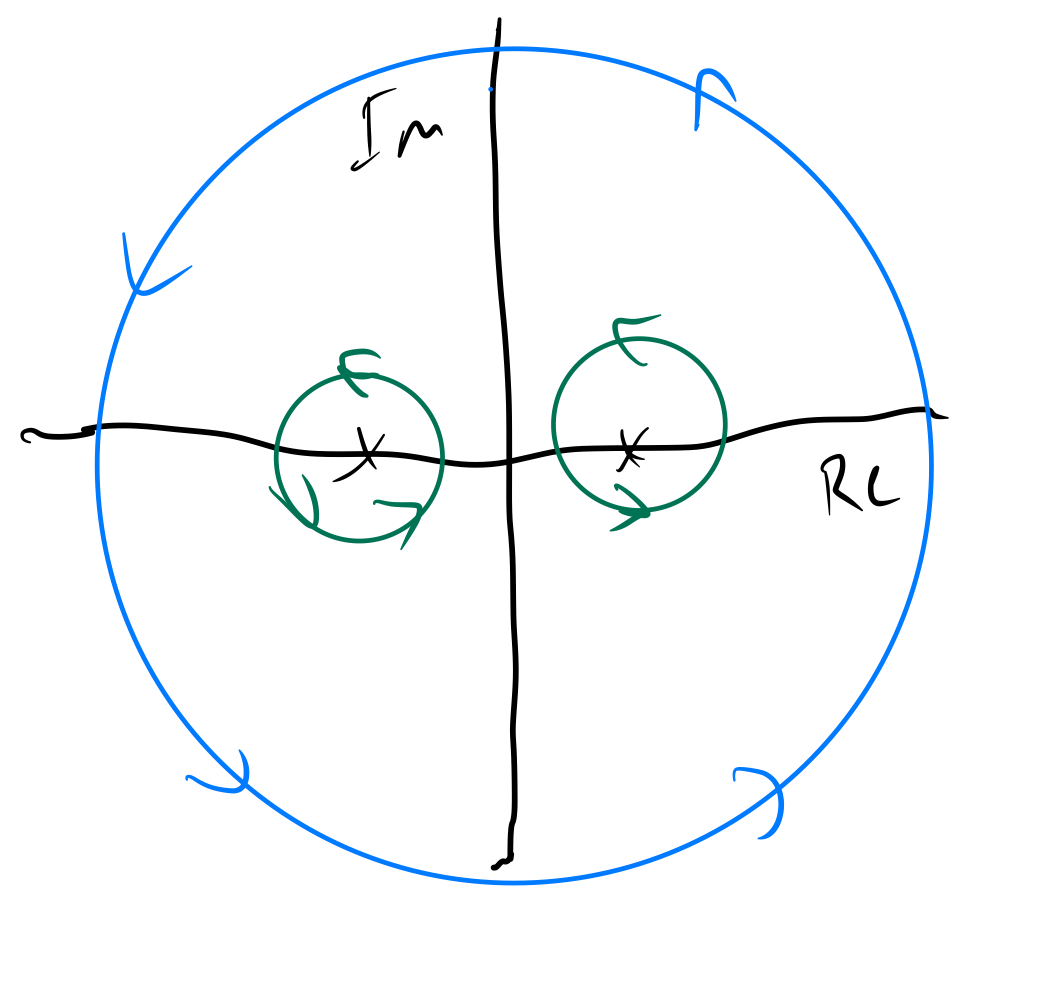
\includegraphics[alt={Curve Around Singularities}]{curve-around-singularities.png}

Now we can find our contour integral by evaluating the contour integrals on paths around our singularities, as these paths are analytic everywhere outside them but inside $C$.

A useful theorem to proceed from here is the following:

\begin{theorem}
If $C$ is a simple, closed, piecewise smooth curve and $z_0$ is interior to $C$, then:

\[ \oint_C \frac{1}{z - z_0} dz = 2 \pi i. \]
\end{theorem}

\begin{intuition}
See \dref{integral-of-one-over-z-around-unit-circle} and consider path independence and the principle of path deformation. Consider toy contours, particularly a collapsed keyhole contour around the singularity.
\end{intuition}

Now, via partial fraction decomposition we have

\[ \oint_C \frac{1}{z^2 - 1} = \frac{1}{2} \oint_C \frac{1}{z-1} - \frac{1}{z+1} dz = \frac{1}{2}\left ( \oint_C \frac{1}{z - 1} dz - \oint_C \frac{1}{z + 1}dz \right ) = \frac{1}{2} \left ( 2 \pi i - 2 \pi i \right ) = 0. \] 

The following theorems illustrate the nice properties of simply connected domains, where we don't have to deal with singularities or holes:

When $f$ is analytic in a simply-connected domain $D$, the contour integral of $f$ around every closed, piecewise smooth curve in $D$ vanishes.

When $f$ is analytic in a simply-connected domain $D$, the contour integral of $f$ is independent of path in $D$.

When $f$ is analytic in a simply-connected domain $D$, it has an antiderivative therein.

\end{document}
